\appendix

\section{Anhang}
\subsection{Speicherung der Daten in eXist}
\begin{figure}[H]
	\centering
		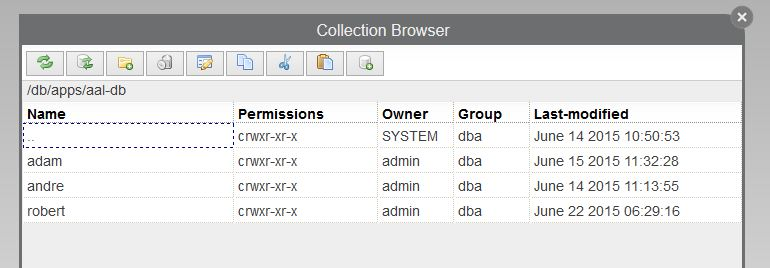
\includegraphics[width=0.8\textwidth]{images/collections1.jpg}
		\caption{Collection für jede Person} 
		\label{collection1}
	\centering
\end{figure}
\begin{figure}[H]
	\centering
		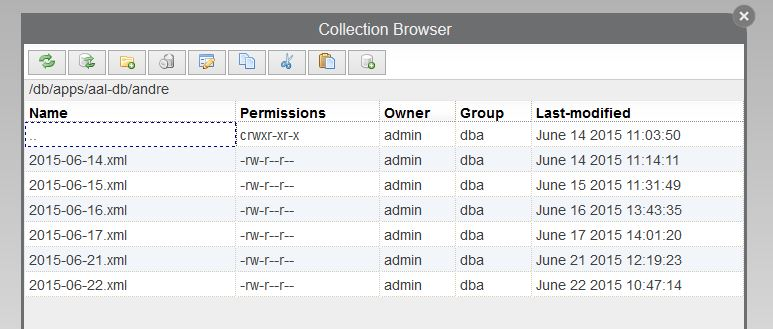
\includegraphics[width=0.8\textwidth]{images/collections2.jpg}
		\caption{XML-Dokument für jeden Tag} 
		\label{collection2}
	\centering
\end{figure}

\subsection{Bedienungsanleitung}
Zunächst muss der Server, auf dem das Projekt gehostet wird, gestartet werden. Dazu öffnet man einen Browser und geht auf die URL http://www.koding.com. Danach muss man sich bei der Website anmelden. Dazu sind folgende Accountdaten einzugeben:

\begin{itemize}
	\item Email address: aal-xml-projekt@web.de
	\item Password: aalxmlprojekt2014
\end{itemize}

Nach der Anmeldung erscheint eine IDE. Es wird ein Fenster angezeigt, mit der Nachricht, dass die koding-vm-0 offline ausgeschaltet ist. Klicken Sie auf den Button \textit{"Turn it on"}. Warten Sie 1-2 Minuten, bis die VM hochgefahren ist. Sollte sich beim Fortschritt nichts mehr tun, laden Sie die Seite neu und versuchen Sie erneut die VM hochzufahren.
\\
\\
Ist die VM hochgefahren und das Fenster ist verschwunden, wird die IDE komplett sichtbar. Rechts neben der Ordnerstruktur befindet sich das Eingabefenster. Klicken Sie in dem Eingabefenster oben oder unten auf das $+$ und gehen in dem sich öffnenden Kontextmenü auf \textit{New Terminal -> New Session}. In dem sich geöffneten Terminalfenster geben Sie bitte ein: \textit{./serverStart.sh} und betätigen Sie Enter. Nach diesem Schritt ist der Node.JS Server und der eXist gestartet.
\\
\\
Danach kann die Seite zur Erzeugung der Sensorwerte unter der URL http://aalxmlprojekt.koding.io/sensor/index.html geöffnet werden.
=======
\subsection{Datengenerator GUI}
\begin{figure}[H]
	\begin{center}
		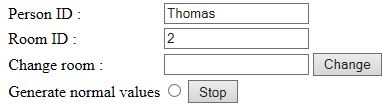
\includegraphics[scale=0.9]{images/eingabe-formular.jpg}
		\caption{Eingabe Formular}
	\end{center}
\end{figure}
\begin{figure}[H]
	\begin{center}
		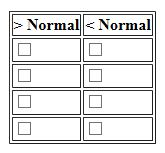
\includegraphics[scale=0.9]{images/kritische-werte-tabelle.jpg}
		\caption{Steuerungsformular}
	\end{center}
\end{figure}
\begin{figure}[H]
	\begin{center}
		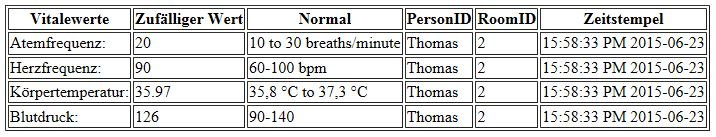
\includegraphics[scale=0.9]{images/vitalwerte-tabelle.jpg}
		\caption{Vitalwerte Tabelle}
	\end{center}
\end{figure}
